\section{Agents}

% ================================================================
\subsection{Class Diagram}

\begin{figure}[H]
  \centering
  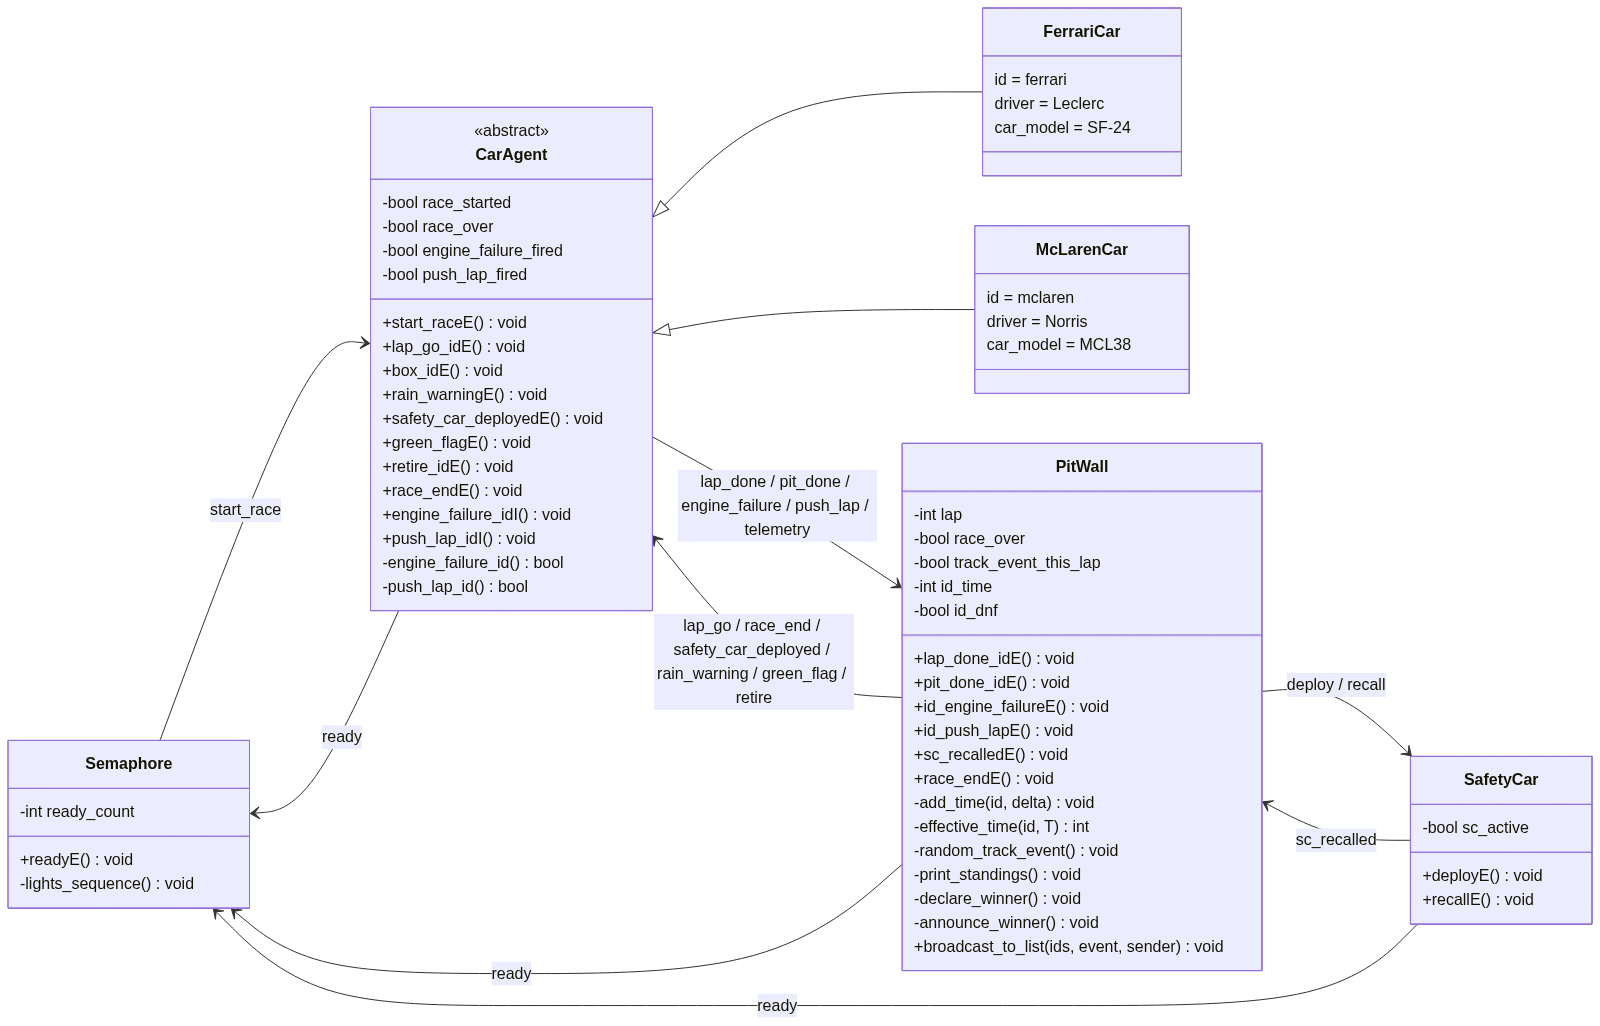
\includegraphics[width=\textwidth]{../../imgs/06_class_diagram.png}
  \caption{Class diagram of the F1 Race MAS.}
  \label{fig:class_diagram}
\end{figure}

The diagram models each DALI agent as a class (or equivalently a \texttt{type}) whose attributes represent its \emph{persistent knowledge base} (Prolog facts asserted at runtime) and whose
operations represent its \emph{reactive} (external) and \emph{proactive}
(internal) event handlers.

\paragraph{CarAgent \textnormal{(one instance per car, dynamically generated)}} 
Holds the per-car racing state:
\texttt{race\_started} and \texttt{race\_over} flags that gate the internal
events; the \texttt{push\_lap\_\{id\}\_fired} flag (reset every lap) that
prevents the push-lap bonus from triggering more than once per lap; and the
\texttt{engine\_failure\_\{id\}\_fired} flag (never reset) that limits the DNF
event to a single occurrence per race.
Its external event handlers react to \texttt{start\_race}, \texttt{lap\_go},
\texttt{pit\_done}, \texttt{race\_end}, \texttt{safety\_car\_deployed},
\texttt{green\_flag} and \texttt{retire}; its internal events
\texttt{engine\_failure\_\{id\}I} and \texttt{push\_lap\_\{id\}I} fire
autonomously when probabilistic conditions are met. \texttt{Id} are used to distinguish between the various instances of the \textit{CarAgent}, such as \textbf{FerrariAgent} and \textbf{McLarenAgent}.

\paragraph{PitWallAgent}
Maintains the authoritative race state: the ordered list of car identifiers
(used for round-robin lap dispatch), the \texttt{lap/1} counter, the
\texttt{effective\_time/2} facts that accumulate each car's total seconds, the
\texttt{track\_event\_this\_lap} flag (prevents more than one track event per
lap), and the \texttt{race\_over} flag.
Its external handlers cover the full race protocol:
\texttt{lap\_done}, \texttt{pit\_done}, \texttt{\{id\}\_engine\_failure},
\texttt{\{id\}\_push\_lap} and \texttt{sc\_recalled}.

\paragraph{SemaphoreAgent}
Counts incoming \texttt{ready} messages via the \texttt{ready\_count/1} fact.
Once the count reaches $N_\text{cars} + 2$ (because the \textit{PitwallAgent} and \textit{SafetyCarAgent} are always present) it runs the lights sequence and
sends \texttt{start\_race} to first car.
It has no internal events.

\paragraph{SafetyCarAgent}
Holds a single boolean fact \texttt{sc\_active} toggled by the
\texttt{deployE} and \texttt{recallE} external events.
On recall it sends \texttt{sc\_recalled} back to the pit wall to trigger the
green-flag chain.

\subsection{DALI semantycs}

\subsubsection{CarAgent: FerrariAgent, McLarenAgent, ...}

The \texttt{FerrariAgent} is the canonical example of a car agent in the
system. Its source file \texttt{mas/types/ferrariCar.txt} is generated by
\texttt{generate\_agents.py} from the \texttt{agents.json} entry for
\texttt{ferrari}. All other car agents follow the same structure with
agent-specific identifiers and driver names substituted.\\

\textbf{Initialisation Directive}

\begin{minipage}{\linewidth}
\begin{lstlisting}[language=Prolog]
:- write('[Ferrari] SF-24 ready on the grid.'),
   send_m(semaphore, send_message(ready, ferrari)).
\end{lstlisting}
\end{minipage}

\noindent
This \emph{directive} (introduced by \texttt{:-}) executes at agent load time, before any event handler is registered. It immediately sends a \texttt{ready} message to the \texttt{semaphore} agent, contributing to the $N_\text{cars}+2$ count that triggers the lights sequence. The four \texttt{dynamic} declarations that follow initialise the agent's mutable knowledge base:

\begin{minipage}{\linewidth}
\begin{lstlisting}[language=Prolog]
:- dynamic race_started/0.
:- dynamic race_over/0.
:- dynamic engine_failure_ferrari_fired/0.
:- dynamic push_lap_ferrari_fired/0.
\end{lstlisting}
\end{minipage}

\noindent
All four facts are absent at startup; they are asserted at runtime by event
handlers and serve as boolean flags.\\

\textbf{External Events}

External events (\texttt{nameE:>~Body.}) are \emph{reactive}: the DALI
runtime fires them whenever a message whose name matches \texttt{name} arrives in the agent's mailbox. \\

\begin{minipage}{\linewidth}
\texttt{start\_raceE} --- Lights Out

\begin{lstlisting}[language=Prolog]
start_raceE:>
    assert(race_started),
    retractall(push_lap_ferrari_fired),
    write('[Ferrari] LAP 1 -- LIGHTS OUT! Leclerc launches off the line!'),
    messageA(pitwall, send_message(lap_done_ferrari, ferrari)).
\end{lstlisting}
\end{minipage}

Sent by the \texttt{semaphore} after the lights-out pause.
\begin{enumerate}[leftmargin=2em, itemsep=2pt]
  \item Asserts \texttt{race\_started}, enabling the internal-event conditions.
  \item Retracts, i.e. removes all clauses that can be unified with the fact, any stale \\ \texttt{push\_lap\_ferrari\_fired} flag (defensive
        reset for the first lap).
  \item Immediately reports the first lap as done to the pit wall via
        \texttt{messageA}.\\
\end{enumerate}

\begin{minipage}{\linewidth}
\texttt{lap\_go\_ferrariE} --- Next Lap Dispatch

\begin{lstlisting}[language=Prolog]
lap_go_ferrariE:>
    if(\+ race_started, assert(race_started), true),
    retractall(push_lap_ferrari_fired),
    write('[Ferrari] On the power! Leclerc attacking every sector.'),
    messageA(pitwall, send_message(lap_done_ferrari, ferrari)).
\end{lstlisting}
\end{minipage}

Sent by the pit wall at the start of every subsequent lap.
\begin{enumerate}[leftmargin=2em, itemsep=2pt]
  \item The \texttt{if} guard handles the edge case where \texttt{start\_race} arrived out of order or was missed: it re-asserts \texttt{race\_started} defensively.
  \item Retracts \texttt{push\_lap\_ferrari\_fired}, resetting the push-lap window so the proactive event can fire again this lap.
  \item Reports the lap immediately as done.
\end{enumerate}

\begin{minipage}{\linewidth}
\texttt{box\_ferrariE} --- Pit Stop
\begin{lstlisting}[language=Prolog]
box_ferrariE:>
   write('[Ferrari] BOX BOX BOX! Ferrari dives into the pits.'),
   messageA(pitwall, send_message(pit_done_ferrari, ferrari)).
\end{lstlisting}
\end{minipage}

Sent by the pit wall when it decides to call Ferrari in for a stop.
Immediately acknowledges the stop with \texttt{pit\_done\_ferrari} so the pit
wall can add the $+25\,\text{s}$ penalty and proceed with lap dispatch.\\

\begin{minipage}{\linewidth}
\texttt{rain\_warningE} and \texttt{safety\_car\_deployedE} --- Track Notifications

\begin{lstlisting}[language=Prolog]
rain_warningE:>
    if(race_over, true,
        (write('[Ferrari] RAIN WARNING. Leclerc switching to intermediate tyres.'), nl)).

safety_car_deployedE:>
    if(race_over, true,
        (write('[Ferrari] Safety car deployed. Leclerc conserving tyres.'), nl)).
\end{lstlisting}
\end{minipage}

Both handlers are \emph{cosmetic}: they never modify the knowledge base and are silently ignored (branch \texttt{true}) if the race has already ended. The \texttt{race\_over} guard prevents spurious output from late-arriving messages after \texttt{race\_endE} has fired.\\

\begin{minipage}{\linewidth}
\texttt{green\_flagE} --- Restart After Safety Car

\begin{lstlisting}[language=Prolog]
green_flagE:>
    if(race_over, true,
        (write('[Ferrari] GREEN FLAG! Leclerc pushing flat out!'), nl)).
\end{lstlisting}
\end{minipage}

Sent by the pit wall once the safety car has been recalled
(\texttt{sc\_recalled} chain). Purely cosmetic; guarded by \texttt{race\_over}.\\

\begin{minipage}{\linewidth}
\texttt{retire\_ferrariE} --- DNF Notification

\begin{lstlisting}[language=Prolog]
retire_ferrariE:>
    write('[Ferrari] *** LECLERC PARKS THE CAR. Ferrari is out of the race. ***').
\end{lstlisting}
\end{minipage}

Sent by the pit wall after receiving an \texttt{engine\_failure} message from
this agent. No state change is needed here because \texttt{race\_over} is only
asserted by \texttt{race\_endE}, which the pit wall broadcasts to all agents
immediately after \texttt{declare\_winner}.\\

\begin{minipage}{\linewidth}
\texttt{race\_endE} --- Race Termination

\begin{lstlisting}[language=Prolog]
race_endE:>
    assert(race_over).
\end{lstlisting}
\end{minipage}

Broadcast by the pit wall to every agent after \texttt{declare\_winner}.
Asserting \texttt{race\_over} causes the conditions of both internal events (\texttt{engine\_failure\_ferrari} and \\\texttt{push\_lap\_ferrari}) to fail permanently, stopping all proactive behaviour.


\textbf{Internal Events}

Internal events (\texttt{nameI:>~Body.}) are \emph{proactive}: the DALI
runtime evaluates the associated condition clause \texttt{name~:-~Cond.} at each agent cycle. If the condition succeeds, the body fires.

\begin{minipage}{\linewidth}
\texttt{engine\_failure\_ferrariI} --- Spontaneous DNF

\begin{lstlisting}[language=Prolog]
engine_failure_ferrari :-
    race_started,
    \+ race_over,
    \+ engine_failure_ferrari_fired,
    random(0, 1000, R), R < 2.

engine_failure_ferrariI:>
    assert(engine_failure_ferrari_fired),
    write('[Ferrari] *** ENGINE FAILURE -- Power loss! Leclerc slowing! ***'),
    send_m(pitwall, send_message(ferrari_engine_failure, ferrari)),
    send_m(pitwall, inform(telemetry(ferrari, engine_failure, critical), ferrari)).
\end{lstlisting}
\end{minipage}

The condition requires four conjuncts to hold simultaneously:
\begin{itemize}[leftmargin=2em, itemsep=2pt]
  \item \texttt{race\_started} --- the race is live.
  \item \texttt{\textbackslash+ race\_over} --- the race has not yet ended.
  \item \texttt{\textbackslash+ engine\_failure\_ferrari\_fired} --- the event has
        not already fired (once-only guard).
  \item \texttt{random(0,\,1000,\,R), R < 2} --- a $0.2\,\%$ probability roll
        succeeds.
\end{itemize}

\noindent
On firing, \texttt{engine\_failure\_ferrari\_fired} is asserted first to
prevent re-entry, then \texttt{send\_m} notifies the pit wall. Note the use of
\texttt{send\_m} (safe inside non-top-level code) rather than
\texttt{messageA} (top-level only). A second \texttt{send\_m} delivers a FIPA
\texttt{inform} with a \texttt{telemetry/3} payload
(\texttt{telemetry(ferrari, engine\_failure, critical)}) at priority~100,
logged by the pit wall as a diagnostic trace. The pit wall reacts via
\texttt{ferrari\_engine\_failureE}, sets the effective time to 9999\,s, and
eventually broadcasts \texttt{race\_end}. \\

\begin{minipage}{\linewidth}
\texttt{push\_lap\_ferrariI} --- Fastest-Lap Bonus

\begin{lstlisting}[language=Prolog]
push_lap_ferrari :-
    race_started,
    \+ race_over,
    \+ push_lap_ferrari_fired,
    random(0, 100, R), R < 10.

push_lap_ferrariI:>
    assert(push_lap_ferrari_fired),
    write('[Ferrari] PUSH LAP! Leclerc going flat out -- setting fastest sectors!'),
    send_m(pitwall, send_message(ferrari_push_lap, ferrari)),
    send_m(pitwall, inform(telemetry(ferrari, push_lap, active), ferrari)).
\end{lstlisting}
\end{minipage}

Structurally identical to the engine-failure event but with a $10\,\%$
probability. The \\ \texttt{push\_lap\_ferrari\_fired} flag is retracted at the
start of every lap by \texttt{lap\_go\_ferrariE} (and \texttt{start\_raceE}),
so the event fires \emph{at most once per lap} rather than at most once per
race. A FIPA \texttt{inform} with payload
\texttt{telemetry(ferrari, push\_lap, active)} is also sent at priority~100
for diagnostic tracing at the pit wall. The pit wall handler subtracts
$3\,\text{s}$ from Ferrari's accumulated time upon receiving
\texttt{ferrari\_push\_lap}.

\textbf{Knowledge Base and Event Summary}

\begin{longtable}{@{} L{0.32\linewidth} L{0.63\linewidth} @{}}
\toprule
\textbf{Name} & \textbf{Description} \\
\midrule
\endhead

\multicolumn{2}{@{}l}{\textit{Knowledge base}} \\[4pt]

\texttt{race\_started} &
Set on lights-out; gates all lap and event handlers \\

\texttt{race\_over} &
Set on \texttt{race\_endE}; silences all guarded handlers \\

\texttt{engine\allowbreak\_failure\allowbreak\_ferrari\allowbreak\_fired} &
One-shot flag; prevents engine-failure from firing twice \\

\texttt{push\_lap\_ferrari\_fired} &
Per-lap flag; retracted by \texttt{lap\_go\_ferrariE} each lap \\

\midrule
\multicolumn{2}{@{}l}{\textit{External events}} \\[4pt]

\texttt{start\_raceE} &
Lights-out from semaphore; asserts \texttt{race\_started}, sends \texttt{lap\_done\_ferrari} \\

\texttt{lap\_go\_ferrariE} &
Pit wall starts a new lap; resets push-lap flag, sends \texttt{lap\_done\_ferrari} \\

\texttt{box\_ferrariE} &
Pit-stop request; sends \texttt{pit\_done\_ferrari} ($+25\,\text{s}$ penalty) \\

\texttt{rain\_warningE} &
Heavy-rain notification (cosmetic, guarded by \texttt{race\_over}) \\

\texttt{safety\_car\_deployedE} &
Safety-car deployment notification (cosmetic, guarded by \texttt{race\_over}) \\

\texttt{green\_flagE} &
Safety-car recalled; car acknowledges green flag (guarded by \texttt{race\_over}) \\

\texttt{retire\_ferrariE} &
DNF confirmation from pit wall; car parks \\

\texttt{race\_endE} &
Race-over broadcast; asserts \texttt{race\_over} \\

\midrule
\multicolumn{2}{@{}l}{\textit{Internal events}} \\[4pt]

\texttt{engine\_failure\_ferrariI} &
$\approx 0.2\,\%$/cycle; fires once per race; notifies pit wall of DNF;
sends \texttt{inform(telemetry(ferrari, engine\_failure, critical))} \\

\texttt{push\_lap\_ferrariI} &
$\approx 10\,\%$/cycle; fires once per lap; deducts $3\,\text{s}$ via pit wall;
sends \texttt{inform(telemetry(ferrari, push\_lap, active))} \\

\bottomrule
\end{longtable}

\newpage
\subsubsection{PitWallAgent}

The \texttt{PitWallAgent} is the race coordinator of the simulation. Its source
file \texttt{mas/\allowbreak types/\allowbreak pitWallType.txt} is generated by \texttt{generate\_agents.py}
and embeds the full car roster: it knows every car by name and drives the
round-robin lap dispatch\footnote{This concept is explained better in Section \ref{sec:round_robin}}. Unlike car agents, it has no internal events: in fact, all its behaviour is reactive.\\

\textbf{Initialisation Directives}

\begin{minipage}{\linewidth}
\begin{lstlisting}[language=Prolog]
:- write('[PitWall] Online.'),
   send_m(semaphore, send_message(ready, pitwall)).
:- dynamic ferrari_time/1.
:- dynamic ferrari_dnf/0.
:- dynamic mclaren_time/1.
:- dynamic mclaren_dnf/0.
:- dynamic lap/1.
:- dynamic race_over/0.
:- dynamic track_event_this_lap/0.
:- assert(ferrari_time(0)).
:- assert(mclaren_time(0)).
:- assert(lap(0)).
\end{lstlisting}
\end{minipage}

\noindent
At load time the agent registers with the semaphore and seeds the knowledge
base. For each car a \texttt{\{id\}\_time/1} accumulator is initialised to
zero and a \texttt{\{id\}\_dnf/0} flag is declared (absent until a DNF
occurs). \texttt{lap/1} holds the current completed-lap count, starting at
zero.\\

\textbf{Knowledge-Base Helpers}

The agent defines three sets of pure Prolog predicates that are called from within event handlers. \\

\begin{minipage}{\linewidth}
\texttt{add\_time/2} and \texttt{effective\_time/2}

\begin{lstlisting}[language=Prolog]
add_time(ferrari, D) :-
    retract(ferrari_time(S)),
    S1 is S + D,
    assert(ferrari_time(S1)).

effective_time(ferrari, T) :- ferrari_dnf, !, T = 9999.
effective_time(ferrari, T) :- ferrari_time(T).
\end{lstlisting}
\end{minipage}

\texttt{add\_time/2} performs an atomic read-modify-write on the accumulator:
it retracts the old value, computes the new one, and re-asserts it. Passing a
negative delta (e.g.\ $-3$) subtracts time. \texttt{effective\_time/2} first
checks the DNF flag with a cut, avoiding the execution of the other predicate; if the car has retired it returns a sentinel
value of 9999 (a simbolic infinite time registered) regardless of the actual accumulator. \\

\begin{minipage}{\linewidth}
\texttt{random\_track\_event/0}

\begin{lstlisting}[language=Prolog]
random_track_event :-
    if(track_event_this_lap, true,
        (random(0, 10, R),
         if(R < 2,
             (assert(track_event_this_lap),
              write('[Race Director] SAFETY CAR deployed. +10s to all.'), nl,
              add_time(ferrari, 10), add_time(mclaren, 10),
              send_m(safety_car, send_message(deploy, pitwall)),
              broadcast_to_list([ferrari, mclaren], safety_car_deployed, pitwall)),
         if(R < 4,
             (assert(track_event_this_lap),
              write('[Race Director] HEAVY RAIN. +5s to all.'), nl,
              add_time(ferrari, 5), add_time(mclaren, 5),
              broadcast_to_list([ferrari, mclaren], rain_warning, pitwall)),
             true)))).
\end{lstlisting}
\end{minipage}

The outer \texttt{if} is an idempotency guard: if \texttt{track\_event\_this\_lap}
is already asserted the predicate returns immediately, ensuring at most one track event per lap. Otherwise a uniform random integer $R \in [0, 10)$ is drawn:
\begin{itemize}[leftmargin=2em, itemsep=2pt]
  \item $R < 2$ ($20\,\%$): safety car deployed, $+10\,\text{s}$ to all cars.
  \item $2 \le R < 4$ ($20\,\%$): heavy rain, $+5\,\text{s}$ to all cars.
  \item $R \ge 4$ ($60\,\%$): no event. \\
\end{itemize}

\begin{minipage}{\linewidth}
\texttt{declare\_winner/0} and \texttt{announce\_winner/0}

\begin{lstlisting}[language=Prolog]
declare_winner :-
    if(race_over, true,
        (assert(race_over),
         write('[PitWall] === CHEQUERED FLAG ==='), nl,
         announce_winner,
         send_m(ferrari, send_message(race_end, pitwall)),
         send_m(mclaren, send_message(race_end, pitwall)))).

announce_winner :-
    findall(T-Id, effective_time(Id, T), Pairs0),
    keysort(Pairs0, Pairs),
    write('[PitWall] === FINAL RESULTS ==='), nl,
    print_podium(Pairs, 1).
\end{lstlisting}
\end{minipage}

\texttt{declare\_winner/0} is guarded by \texttt{race\_over} to prevent double
invocation (it can be triggered by either the last \texttt{lap\_done} or an
engine-failure event). It asserts \texttt{race\_over}, prints the podium via
\texttt{announce\_winner/0}, and broadcasts \texttt{race\_end} to all cars
using \texttt{broadcast\_to\_list/3} (defined in \texttt{communication.con})
instead of individual \texttt{send\_m} calls, so the number of cars is never
hardcoded here.
\texttt{announce\_winner/0} uses \texttt{findall} to collect all
\texttt{effective\_time} pairs, sorts them by key (time) with
\texttt{keysort}, and delegates formatted output to \texttt{print\_podium/2}.\\

\textbf{External Events}

\begin{minipage}{\linewidth}
\texttt{lap\_done\_ferrariE} --- Ferrari Lap Completion

\begin{lstlisting}[language=Prolog]
lap_done_ferrariE:>
    if(race_over, true,
        (random(60, 91, T),
         add_time(ferrari, T),
         write('[PitWall] Ferrari lap: '), write(T), write('s'), nl,
         random_track_event,
         messageA(mclaren, send_message(lap_go_mclaren, pitwall)))).
\end{lstlisting}
\end{minipage}

Triggered when Ferrari reports a completed lap.
\begin{enumerate}[leftmargin=2em, itemsep=2pt]
  \item Draws a random lap time $T \in [60, 90]\,\text{s}$ and adds it to Ferrari's accumulator.
  \item Calls \texttt{random\_track\_event} to potentially inject a safety car or rain event.
  \item Dispatches the next lap token to McLaren via \texttt{messageA}.\\
\end{enumerate}

\begin{minipage}{\linewidth}
\texttt{lap\_done\_mclarenE} --- McLaren Lap Completion and Lap Counter

\begin{lstlisting}[language=Prolog]
lap_done_mclarenE:>
    if(race_over, true,
        (random(60, 91, T),
         add_time(mclaren, T),
         write('[PitWall] McLaren lap: '), write(T), write('s'), nl,
         (track_event_this_lap
             -> (retract(track_event_this_lap),
                 send_m(safety_car, send_message(recall, pitwall)))
             ; true),
         retract(lap(N)), N1 is N + 1, assert(lap(N1)),
         write('[PitWall] Lap '), write(N1), write(' / 5'), nl,
         print_standings,
         if(N1 =:= 5, declare_winner,
             (random_track_event,
              messageA(ferrari, send_message(lap_go_ferrari, pitwall)))))).
\end{lstlisting}
\end{minipage}

McLaren is last in the round-robin, so this handler carries the end-of-lap bookkeeping:
\begin{enumerate}[leftmargin=2em, itemsep=2pt]
  \item Adds McLaren's lap time.
  \item If a track event occurred this lap, retracts the flag and sends
        \texttt{recall} to the safety car (triggering the \texttt{sc\_recalled}
        chain).
  \item Increments the lap counter and prints the current standings.
  \item If the total lap count equals 5, calls \texttt{declare\_winner};
        otherwise rolls another \texttt{random\_\allowbreak track\_\allowbreak event} and dispatches
        \texttt{lap\_go\_ferrari} to start the next lap. \\
\end{enumerate}

\begin{minipage}{\linewidth}
\texttt{pit\_done\_ferrariE} and \texttt{pit\_done\_mclarenE} --- Pit Stops

\begin{lstlisting}[language=Prolog]
pit_done_ferrariE:>
    if(race_over, true,
        (add_time(ferrari, 25),
         write('[PitWall] Ferrari pit stop +25s.'), nl,
         messageA(mclaren, send_message(lap_go_mclaren, pitwall)))).

pit_done_mclarenE:>
    if(race_over, true,
        (add_time(mclaren, 25),
         write('[PitWall] McLaren pit stop +25s.'), nl,
         retract(lap(N)), N1 is N + 1, assert(lap(N1)),
         if(N1 =:= 5, declare_winner,
             messageA(ferrari, send_message(lap_go_ferrari, pitwall))))).
\end{lstlisting}
\end{minipage}

Each handler adds the $+25\,\text{s}$ pit-stop penalty and then resumes the
round-robin exactly as its \texttt{lap\_done} counterpart would. Note that
\texttt{pit\_done\_mclarenE} also increments the lap counter because a pit
stop replaces the normal lap-done report for the last car in the round.\\

\begin{minipage}{\linewidth}
\texttt{sc\_recalledE} --- Safety Car Recalled

\begin{lstlisting}[language=Prolog]
sc_recalledE:>
    write('[Race Director] GREEN FLAG! Track is clear.'), nl,
    broadcast_to_list([ferrari, mclaren], green_flag, pitwall).
\end{lstlisting}
\end{minipage}

Sent by the \texttt{SafetyCarAgent} after receiving \texttt{recall}. The pit
wall announces the green flag and forwards it to every car so their
\texttt{green\_flagE} handlers can fire.\\

\begin{minipage}{\linewidth}
\texttt{ferrari\_engine\_failureE} and \texttt{mclaren\_engine\_failureE} --- DNF

\begin{lstlisting}[language=Prolog]
ferrari_engine_failureE:>
    assert(ferrari_dnf),
    write('[PitWall] Ferrari DNF. Leclerc is out.'), nl,
    send_m(ferrari, send_message(retire_ferrari, pitwall)),
    declare_winner.

mclaren_engine_failureE:>
    assert(mclaren_dnf),
    write('[PitWall] McLaren DNF. Norris is out.'), nl,
    send_m(mclaren, send_message(retire_mclaren, pitwall)),
    declare_winner.
\end{lstlisting}
\end{minipage}

Triggered by a car's \texttt{engine\_failure\_\{id\}I} internal event. The
handler asserts the DNF flag (causing \texttt{effective\_time} to return 9999
for that car), sends the cosmetic \texttt{retire\_\{id\}} message back to the car, and calls \texttt{declare\_winner} immediately, ending the race for all
participants.\footnote{This is a known limitation of the current implementation: any DNF unconditionally terminates the entire race, regardless of how many cars are still running. A more realistic design would call \texttt{declare\_winner} only when all but one car have retired, and would remove the DNF car from the round-robin dispatch chain. Both changes would require the \texttt{PitWallAgent} to maintain a dynamic list of active cars rather than a hardcoded sequence of named message sends.}\\

\begin{minipage}{\linewidth}
\texttt{ferrari\_push\_lapE} and \texttt{mclaren\_push\_lapE} --- Fastest Lap Bonus

\begin{lstlisting}[language=Prolog]
ferrari_push_lapE:>
    if(race_over, true,
        (add_time(ferrari, -3),
         write('[PitWall] Ferrari fastest lap! -3s'), nl)).

mclaren_push_lapE:>
    if(race_over, true,
        (add_time(mclaren, -3),
         write('[PitWall] McLaren fastest lap! -3s'), nl)).
\end{lstlisting}
\end{minipage}

Triggered by a car's \texttt{push\_lap\_\{id\}I} internal event. Calls
\texttt{add\_time} with $\Delta = -3$ to subtract three seconds from the
car's accumulator. Guarded by \texttt{race\_over} to ignore late-arriving
push-lap messages after the race has ended. \\

\textbf{Knowledge Base and Event Summary}

\begin{longtable}{@{} l l @{}}
\toprule
\textbf{Name} & \textbf{Description} \\
\midrule
\endhead

\multicolumn{2}{@{}l}{\textit{Knowledge base}} \\[4pt]

\texttt{ferrari\_time/1}         & Accumulated race time for Ferrari (seconds) \\
\texttt{mclaren\_time/1}         & Accumulated race time for McLaren (seconds) \\
\texttt{ferrari\_dnf/0}          & Asserted on engine failure; makes \texttt{effective\_time} return 9999 \\
\texttt{mclaren\_dnf/0}          & Asserted on engine failure; makes \texttt{effective\_time} return 9999 \\
\texttt{lap/1}                   & Current completed-lap counter; starts at 0 \\
\texttt{race\_over/0}            & Asserted by \texttt{declare\_winner}; gates all handlers \\
\texttt{track\_event\_this\_lap/0} & One-shot flag; prevents multiple track events per lap \\

\midrule
\multicolumn{2}{@{}l}{\textit{External events}} \\[4pt]

\texttt{lap\_done\_ferrariE}         & Adds lap time, rolls track event, dispatches to McLaren \\
\texttt{lap\_done\_mclarenE}         & Adds lap time, recalls SC if needed, increments lap, checks race end \\
\texttt{pit\_done\_ferrariE}         & Adds $+25\,\text{s}$, dispatches to McLaren \\
\texttt{pit\_done\_mclarenE}         & Adds $+25\,\text{s}$, increments lap, checks race end \\
\texttt{sc\_recalledE}               & Safety car recalled; broadcasts \texttt{green\_flag} to all cars via \texttt{broadcast\_to\_list} \\
\texttt{ferrari\_engine\_failureE}   & Asserts DNF, retires car, triggers \texttt{declare\_winner} \\
\texttt{mclaren\_engine\_failureE}   & Asserts DNF, retires car, triggers \texttt{declare\_winner} \\
\texttt{ferrari\_push\_lapE}         & Subtracts $3\,\text{s}$ from Ferrari's accumulator \\
\texttt{mclaren\_push\_lapE}         & Subtracts $3\,\text{s}$ from McLaren's accumulator \\

\bottomrule
\end{longtable}

% ----------------------------------------------------------------
\subsubsection{SemaphoreAgent}

The \texttt{SemaphoreAgent} is the race starter. Its source file
\texttt{mas/types/semaphoreType.txt} is generated by
\texttt{generate\_agents.py} and encodes the exact number of agents that
must check in before the lights sequence can begin. It has no internal
events and only one external event handler.\\

\textbf{Initialisation Directives}

\begin{minipage}{\linewidth}
\begin{lstlisting}[language=Prolog]
:- write('Semaphore: Waiting for all F1 agents to be ready...'), nl.
:- dynamic ready_count/1.
:- if(clause(ready_count(_), _), true, assert(ready_count(0))).
\end{lstlisting}
\end{minipage}

\noindent
The agent declares a single mutable counter \texttt{ready\_count/1} and
initialises it to 0 only if it is not already present. The
\texttt{if(clause(\ldots),\,true,\,assert(\ldots))} idiom is a safe
guard against double-initialisation that could arise if the directive were
executed more than once.\\

\textbf{Knowledge-Base Helper}

\begin{minipage}{\linewidth}
\texttt{lights\_sequence/0}

\begin{lstlisting}[language=Prolog]
lights_sequence :-
    write('Semaphore: ========================================'), nl,
    write('Semaphore: F1 RACE START SEQUENCE INITIATED'), nl,
    write('Semaphore: ========================================'), nl,
    sleep(1), write('Semaphore:  (O) ( ) ( ) ( ) ( )  -- light 1'), nl,
    sleep(1), write('Semaphore:  (O) (O) ( ) ( ) ( )  -- light 2'), nl,
    sleep(1), write('Semaphore:  (O) (O) (O) ( ) ( )  -- light 3'), nl,
    sleep(1), write('Semaphore:  (O) (O) (O) (O) ( )  -- light 4'), nl,
    sleep(1), write('Semaphore:  (O) (O) (O) (O) (O)  -- light 5'), nl,
    sleep(2), write('Semaphore:  *** LIGHTS OUT! ***'), nl,
    write('Semaphore:  ( ) ( ) ( ) ( ) ( )  -- GO GO GO!'), nl,
    write('Semaphore: ========================================'), nl,
    send_m(ferrari, send_message(start_race, semaphore)).
\end{lstlisting}
\end{minipage}

The predicate implements the canonical F1 start procedure: five red lights
come on one per second ($5 \times 1\,\text{s}$), hold for
$2\,\text{s}$, then go out. All timing is achieved with blocking
\texttt{sleep/1} calls, which is acceptable here because the semaphore has
no other concurrent duties once the lights are running. On completion it
sends \texttt{start\_race} to the first car (\texttt{ferrari}), which
triggers the round-robin lap dispatch.\\

\textbf{External Events}

\begin{minipage}{\linewidth}
\texttt{readyE} --- Agent Registration

\begin{lstlisting}[language=Prolog]
readyE:>
    retract(ready_count(N)),
    retractall(ready_count(_)),
    N1 is N + 1,
    assert(ready_count(N1)),
    write('Semaphore: '), write(N1), write('/'), write(4),
    write(' agents ready.'), nl,
    if(N1 =:= 4, lights_sequence, true).
\end{lstlisting}
\end{minipage}

Sent by every agent at load time (cars, pit wall, safety car). Each arrival:
\begin{enumerate}[leftmargin=2em, itemsep=2pt]
  \item \texttt{retract(ready\_count(N))} removes one clause and binds \texttt{N}
        to the current value, necessary because \texttt{retractall} discards
        clauses without binding any variable and therefore cannot be used alone
        to read the counter. The subsequent \texttt{retractall(ready\_count(\_))}
        then eliminates any duplicate clauses that may have accumulated if two
        \texttt{ready} messages were processed concurrently before either had
        time to run its own \texttt{retract}.
  \item Increments the counter and re-asserts it.
  \item Prints the current progress (e.g.\ \texttt{2/4 agents ready}).
  \item When the count reaches the threshold (here hardcoded to 4, generated
        from \texttt{agents.json} as $N_\text{cars} + 2$), calls
        \texttt{lights\_sequence/0} to start the race; otherwise waits for
        the next \texttt{ready} message.
\end{enumerate}

\textbf{Knowledge Base and Event Summary}

\begin{longtable}{@{} l l @{}}
\toprule
\textbf{Name} & \textbf{Description} \\
\midrule
\endhead

\multicolumn{2}{@{}l}{\textit{Knowledge base}} \\[4pt]

\texttt{ready\_count/1} & Running count of \texttt{ready} signals received; initialised to 0 \\

\midrule
\multicolumn{2}{@{}l}{\textit{External events}} \\[4pt]

\texttt{readyE} & Increments the counter; fires \texttt{lights\_sequence} when threshold is reached \\

\bottomrule
\end{longtable}

% ----------------------------------------------------------------
\subsubsection{SafetyCarAgent}

The \texttt{SafetyCarAgent} is the simplest agent in the system. Its source
file \texttt{mas/\allowbreak types/\allowbreak safetyCarType.txt} is generated by
\texttt{generate\_agents.py}. It manages a single boolean flag
(\texttt{sc\_active}) and acts as a stateful relay in the safety-car
message chain between the pit wall and the car agents.\\

\textbf{Initialisation Directives}

\begin{minipage}{\linewidth}
\begin{lstlisting}[language=Prolog]
:- write('Safety Car ready. Standing by.'), nl,
   send_m(semaphore, send_message(ready, safety_car)).
:- dynamic sc_active/0.
\end{lstlisting}
\end{minipage}

\noindent
At load time the agent registers with the semaphore and declares the
\texttt{sc\_active/0} flag, which is absent until a \texttt{deploy} message
arrives.\\

\textbf{External Events}

\begin{minipage}{\linewidth}
\texttt{deployE} --- Safety Car Deployment

\begin{lstlisting}[language=Prolog]
deployE:>
    if(sc_active, true,
        (assert(sc_active),
         write('SAFETY CAR: DEPLOYED! Yellow flags! All cars reduce speed!'), nl)).
\end{lstlisting}
\end{minipage}

Sent by the pit wall when \texttt{random\_track\_event} rolls a safety-car
result. The \texttt{if(sc\_active,\,true,\,...)} guard makes the handler
idempotent: if the safety car is already deployed a second \texttt{deploy}
message is silently ignored. Otherwise \texttt{sc\_active} is asserted and
the deployment is logged.\\

\begin{minipage}{\linewidth}
\texttt{recallE} --- Safety Car Recalled

\begin{lstlisting}[language=Prolog]
recallE:>
    if(sc_active,
        (retract(sc_active),
         write('SAFETY CAR: Returning to pits. Notifying race control.'), nl,
         send_m(pitwall, send_message(sc_recalled, safety_car))),
        true).
\end{lstlisting}
\end{minipage}

Sent by the pit wall at the end of the lap during which the safety car was
deployed. The guard here is inverted: the recall is only processed if the
safety car is actually active. On recall:
\begin{enumerate}[leftmargin=2em, itemsep=2pt]
  \item \texttt{sc\_active} is retracted, clearing the deployment state.
  \item \texttt{sc\_recalled} is sent back to the pit wall, triggering
        \texttt{sc\_recalledE} there, which in turn broadcasts
        \texttt{green\_flag} to all cars.
\end{enumerate}
This completes the three-step safety-car chain:
\texttt{random\_track\_event} (PitWall) $\to$ \texttt{recallE} (SafetyCar) $\to$
\texttt{sc\_recalledE} (PitWall) $\to$ \texttt{green\_flagE} (CarAgents).\\

\textbf{Knowledge Base and Event Summary}

\begin{longtable}{@{} l l @{}}
\toprule
\textbf{Name} & \textbf{Description} \\
\midrule
\endhead

\multicolumn{2}{@{}l}{\textit{Knowledge base --- dynamic facts}} \\[4pt]

\texttt{sc\_active/0} & Present while the safety car is deployed; absent otherwise \\

\midrule
\multicolumn{2}{@{}l}{\textit{External events}} \\[4pt]

\texttt{deployE}          & Asserts \texttt{sc\_active}; idempotent if already deployed \\
\texttt{recallE}          & Retracts \texttt{sc\_active}, sends \texttt{sc\_recalled} to pit wall \\

\bottomrule
\end{longtable}

% ----------------------------------------------------------------
\subsection{Custom FIPA Primitives (\texttt{communication.con})}
\label{sec:fipa_primitives}

The file \texttt{conf/communication.con} extends the standard set of DALI
\texttt{told}/\texttt{tell} rules with two F1-specific FIPA primitives.
Both are active for every agent in the MAS because \texttt{communication.con}
is loaded globally at agent startup.

\subsubsection{\texttt{broadcast\_to\_list/3} --- One-to-Many Inform}

\begin{minipage}{\linewidth}
\begin{lstlisting}[language=Prolog]
broadcast_to_list([], _, _).
broadcast_to_list([H|T], Content, Sender) :-
    send_m(H, send_message(Content, Sender)),
    broadcast_to_list(T, Content, Sender).

told(Ag, inform(broadcast(Targets, Content, Sender)), 70) :-
    write('[Broadcast] from '), write(Sender), write(' to '), write(Targets), nl,
    write('[Broadcast] content: '), write(Content), nl,
    broadcast_to_list(Targets, Content, Sender),
    !.

tell(To, _, inform(broadcast(_, _, _))) :- true.
\end{lstlisting}
\end{minipage}

\noindent
A recursive helper that sends the same \texttt{send\_message} to every agent
in \texttt{Targets}. The companion \texttt{told/3} rule at priority~70 (equal
to the standard \texttt{inform} priority) handles the case where an agent
\emph{receives} an \texttt{inform(broadcast(\ldots))} message, it logs the
broadcast and delegates to the helper, cutting after the first successful
match.

In the generated \texttt{pitWallType.txt}, every multi-car notification is
expressed with this primitive rather than with repeated individual
\texttt{send\_m} calls:

\begin{minipage}{\linewidth}
\begin{lstlisting}[language=Prolog]
broadcast_to_list([ferrari, mclaren], safety_car_deployed, pitwall).
broadcast_to_list([ferrari, mclaren], rain_warning,        pitwall).
broadcast_to_list([ferrari, mclaren], green_flag,          pitwall).
broadcast_to_list([ferrari, mclaren], race_end,            pitwall).
\end{lstlisting}
\end{minipage}

\noindent
Because the list is built from \texttt{agents.json} at generation time, adding
or removing a car from the roster requires no manual edits to the broadcast
calls.

\subsubsection{\texttt{inform(telemetry/3)} --- Diagnostic Telemetry}

\begin{minipage}{\linewidth}
\begin{lstlisting}[language=Prolog]
told(Ag, inform(telemetry(Car, Data, Level)), 100) :-
    write('[Telemetry] '), write(Car),
    write(' | '), write(Data),
    write(' | '), write(Level), nl,
    !.

tell(To, _, inform(telemetry(_, _, _))) :- true.
\end{lstlisting}
\end{minipage}

\noindent
A high-priority (\texttt{100}) \texttt{told} rule that intercepts any
\texttt{inform} whose content is a \texttt{telemetry/3} term.  The three
arguments are:
\begin{itemize}[leftmargin=2em, itemsep=2pt]
  \item \texttt{Car}: the originating car identifier (\emph{e.g.}\ \texttt{ferrari}).
  \item \texttt{Data}: the event type (\texttt{engine\_failure} or \texttt{push\_lap}).
  \item \texttt{Level}: severity or mode (\texttt{critical} or \texttt{active}).
\end{itemize}

Car agents send this message alongside the standard \texttt{send\_message} in
their \texttt{engine\_failure\_\{id\}I} and \texttt{push\_lap\_\{id\}I}
handlers.  The receiving agent (pit wall) logs the payload via \texttt{write}
and stores it in its \texttt{past\_event} database via the standard
\texttt{call\_inform} infrastructure.  No reactive logic is currently
triggered on receipt; the record can be queried retrospectively.
